\newcommand{\files}[1]{
    \hfill
    \mbox{
        $\hookrightarrow$
        \texttt{#1}
    }
}

\section{Lautsprecher}
\label{sec:1}
In dieser Aufgabe werden die Schallabstrahlungsmuster einer Quelle visualisiert sowie der Frequenzgang zweier Lautsprecher zum einen linearisiert und zum anderen modelliert.


\subsection{Abstrahlcharakteristik}
\label{subsec:a}
Abbildung \ref{fig:balloon} zeigt die Abstrahlcharakteristik eines Cellos bei verschiedenen Frequenzen in Oktavabstand.
Für eine anschauliche Darstellung wurden die Werte so normiert, dass der niedrigste Wert auf 20 dB liegt.
Mit steigender Frequenz ist zu erkennen, dass die Schalldruckpegelwerte im allgemeinem abnehmen.
Darüber hinaus deformiert sich die zunächst sphärische Form des Ballons zu den hohen Frequenzen hin mit hervortretenden bzw. hineinragenden Beulen.
Daher scheint die Ausbreitung der Schalldruckpegel bei niedrigen Frequenzen nahezu kugelförmig zu sein.
Bei hohen Frequenzen wird zunehmend die für ein Cello charakteristische Abstrahlrichtung erkennbar - leicht schräg nach oben (orthogonal zu den F-Löchern des Resonanzkörpers) und horizontal in die Breite gehend.
Schallabsorbierende Hindernisse vom Cellisten und dem Cello selbst haben auch Einfluss auf die Ausbreitung des Schalldruckpegel.
So ist über alle Frequenzen hinweg ein Abfall des Schalldruckpegel nach hinten, im Schatten des Cellisten, erkennbar.
Bei hohen Frequenzen mit kurzer Wellenlänge lässt sich eine kleine Lücke, vermutlich durch die spielende Hand mit Arm und den Bogen verursacht, vermuten.
\files{main.m, balloonplot.m}


\begin{figure}[h!]
    \centering
    \begin{subfigure}{.5\textwidth}
        \centering
        \caption{125 Hz}
        \includegraphics[width=0.80\linewidth]{Figures/125Hz.eps}
    \end{subfigure}%
    \begin{subfigure}{.5\textwidth}
        \centering
        \caption{250 Hz}
        \includegraphics[width=0.80\linewidth]{Figures/250Hz.eps}
    \end{subfigure}

    \vspace{0.5cm}
    \begin{subfigure}{.5\textwidth}
        \centering
        \caption{500 Hz}
        \includegraphics[width=0.80\linewidth]{Figures/500Hz.eps}
    \end{subfigure}%
    \begin{subfigure}{.5\textwidth}
        \centering
        \caption{1000 Hz}
        \includegraphics[width=0.80\linewidth]{Figures/1000Hz.eps}
    \end{subfigure}

    \vspace{0.5cm}
    \begin{subfigure}{.5\textwidth}
        \centering
        \caption{2000 Hz}
        \includegraphics[width=0.80\linewidth]{Figures/2000Hz.eps}
    \end{subfigure}%
    \begin{subfigure}{.5\textwidth}
        \centering
        \caption{4000 Hz}
        \includegraphics[width=0.80\linewidth]{Figures/4000Hz.eps}
    \end{subfigure}

    \vspace{0.5cm}
    \begin{subfigure}{.5\textwidth}
        \centering
        \caption{8000 Hz}
        \includegraphics[width=0.80\linewidth]{Figures/8000Hz.eps}
    \end{subfigure}

    \caption{Abstrahlcharakteristik eines Cellos bei verschiedenen Frequenzen in Oktavabstand}
    \label{fig:balloon}
\end{figure}


\subsection{Frequenzgang}
\label{subsec:b}
Um den Frequenzgang und die passende Abtastfrequenz $f_s$ des Lautsprechers Adam A7 zu erhalten, verwenden wir die Funktion \textit{read\_spk.m}.
Das Spektrum enthält Informationen über den Frequenzbereich zwischen 1 und 24000 Hz.
Die obere Grenze entspricht dabei der halben Abtastfrequenz und die Frequenzauflösung bzw. Frequenzschrittweite ist $\Delta f = f_s / N$, wobei N die doppelte Länge des Vektors mit Informationen über den gemessenen Frequenzgang ist, also $N = 2 \cdot 16385$.
Für die grafische Darstellung des Betragsfrequenzgangs normieren wir alle Amplitudenwerte auf den Wert bei 1000 Hz.
Zudem rechnen wir die Werte in Pegelwerte um, was äquivalent zu einer grafischen Logarithmierung der y-Achse ist.
Dabei entsprechen 0 dB wiederum dem Wert bei 1000 Hz.
Das Resultat ist in den Abbildungen \ref{fig:frequenzgangA7} und \ref{fig:frequenzgangA7_lin} dargestellt. 
In Abbildung \ref{fig:frequenzgangA7} ist zu sehen, dass der Lautsprecher bis zu einer Frequenz von ca. 20 kHz vermessen wurde, die Werte danach enthalten keinen Informationsgehalt mehr.\\
Der theoretische Frequenzgang eines elektrodynamischen Lautsprechers steigt bei tiefen Frequenzen zunächst an bis zur Resonanzfrequenz des Lautsprechers, bei welcher eine Überhöhung zu erkennen ist.
Dann folgt ein linearer Bereich, der sich bis zur oberen Grenzfrequenz erstreckt, der Knickfrequenz, ab der der Frequenzgang zu hohen Frequenzen hin abfällt. 
In Fall des Adam A7 liegt die Resonanzfrequenz bei etwa 100 Hz.
Der für die Knickfrequenz charakteristische Abfall ist nicht zu erkennen, was dafür spricht, dass die Knickfrequenz außerhalb des vermessenen Bereichs liegt.
Es ist sinnvoll einen Lautsprecher so zu entwickeln, dass sich der lineare Bereich bis zu möglichst hohen Frequenzen erstreckt und die Knickfrequenz außerhalb des hörbaren Bereichs liegt.
Weiterhin fällt auf, dass der lineare Bereich nur annähernd linear ist und viele Störungen enthält.\\

\begin{figure}[H]
        \centering
        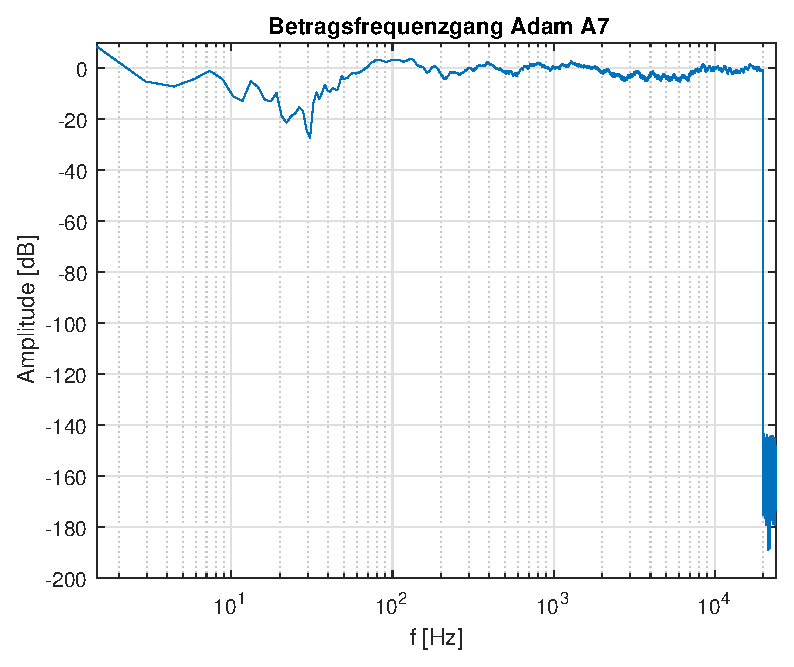
\includegraphics[width=0.7\textwidth]{Figures/frequenzgangA7.eps}
        \caption{Messdaten für den Frequenzgang des Lautsprechers Adam A7 im Bereich 0 bis 24000 Hz}
        \label{fig:frequenzgangA7}
\end{figure}

Als nächstes erweitern wir den gemessenen Frequenzgang um die komplex konjugierte Spiegelung. 
Dieses Spektrum, welches nun Werte von 0 bis 48000 Hz enthält, kann durch inverse Fouriertransformation in den Zeitbereich abgebildet werden.
Der Realteil des Ergebnisses liefert uns die Impulsantwort.
Mithilfe der Funktion \textit{peq.m} können wir verschiedene parametrische Filter auf die Impulsantwort anwenden und diese danach mittels einer FFT wieder in den Frequenzbereich transformieren, um den Betragsfrequenzgang des Lautsprechers zu linearisieren.
Insgesamt haben wir 13 Filter angewendet um auf das in Abbildung \ref{fig:frequenzgangA7_lin} dargestellte Resultat zu kommen.
Die Parameter der verwendeten Filter sind in Tabelle \ref{tab:filterparameter} zu sehen.\\
\files{main.m, read\_spk.m, itafread.com, peq.m}

\begin{table}[H]
    \centering
    \caption{Filterparameter}
    \label{tab:filterparameter}
    \begin{tabular}{| c |c |c |}
    	\hline
        Mittenfrequenz [Hz] & Verstärkung [dB] & Güte\\
        \hline
        25 & 15 & 1 \\
		29.5 & 20 & 15 \\
		100 & -5 & 1\\
		200 & 4 & 2\\
		400 & -3 & 1 \\
		600 & 5 & 1\\
		700 &-2 & 1 \\
		800 & -2 & 3\\
		1000 & 2 & 1\\
		1200 & -4 & 1\\
		4000 & 3 & 0.5\\
		6000 & 1 & 1\\
		8500 & -3 & 2\\
        \hline
    \end{tabular}
\end{table}

\begin{figure}[H]
        \centering
        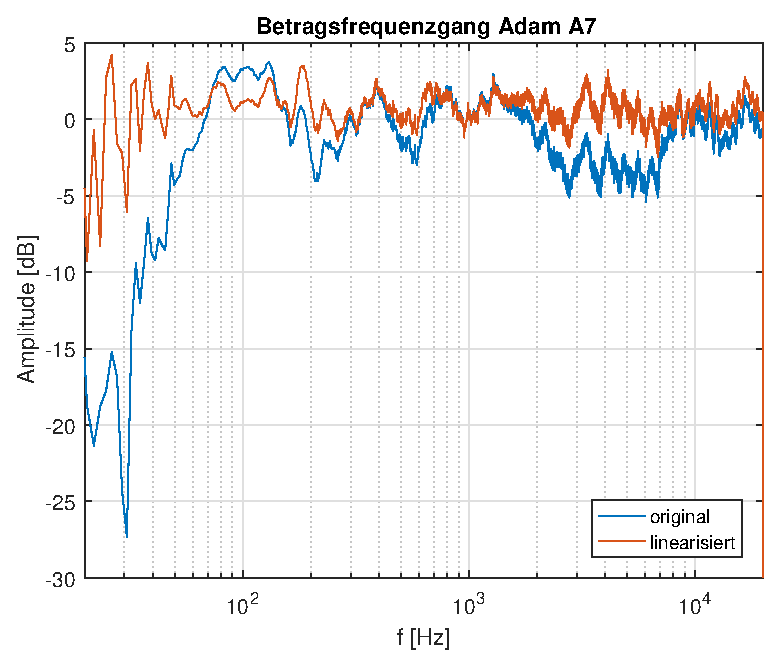
\includegraphics[width=0.7\textwidth]{Figures/frequenzgangA7_lin.eps}
        \caption{Linearisierter und Originalbetragsfrequenzgang für den Bereich 20 Hz bis 20000 Hz}
        \label{fig:frequenzgangA7_lin}
\end{figure}




\subsection{SPH-450TC Treiber}
\label{subsec:c}

Die zur Berechnung des Frequenzgangs benötigten Thiele-Small-Parameter wurden dem Datenblatt \cite{SPH-450TC} des SPH-450TC Treibers entnommen.

\begin{itemize}
  \item Resonanzfrequenz $f_s$ = 20 Hz
  \item Gesamtgüte $Q_{ts}$ = 0,25
  \item Äquivalentvolumen $V_{as}$ = 480 l
\end{itemize}

Mit Hilfe von Formel \ref{eq:f1} wurde die Resonanzkreisfrequenz $\omega_c$ berechnet.
Wie gefordert wurde für $Q_{ts}$ der Wert $\frac{1}{\sqrt{2}}$ verwendet.

\begin{align}
\label{eq:f1}
\omega_c = \frac{Q_{tc}}{Q_{ts}} \cdot \omega_s 
\end{align}

Die Lösung der Gleichung ergab ein $\omega_c$ von $355.4 \frac{1}{s}$ ($f_c = 56.5$ Hz). 
Mit diesem Ergebnis und den Werten aus dem Datenblatt lässt sich nun das benötigte Gehäusevolumen mittels Gleichung \ref{eq:f2} errechnen.

\begin{align}
\label{eq:f2}
V_b = \frac{V_{as}} {\left( \frac{\omega_c}{\omega_s} \right) ^{2} - 1}
\end{align}

Das berechnete Gehäusevolumen  $V_b$ beträgt 68,57 Liter.
Der mittels Formel \ref{eq:f3} berechnete modellhafte Amplitudenfrequenzgang ist in Abbildung \ref{fig:Normaler_Frequenzgang} zu sehen.

\begin{align}
\label{eq:f3}
G(\omega) = \frac{(\frac{\omega}{\omega_c})^2}{(\frac{\omega}{\omega_c})^2 - j \frac{1}{Q_{tc}}\frac{\omega}{\omega_c}-1}
\end{align}
Die Resonanzfrequenz $f_c$ wurde in der Abbildung mit einem roten Kreis markiert. 
Die -3 dB Cutoff-Frequenz wurde mit einem roten Sternchen markiert.
In diesem Fall liegen beide Werte aufeinander.

\begin{figure}[H]
    \centering
    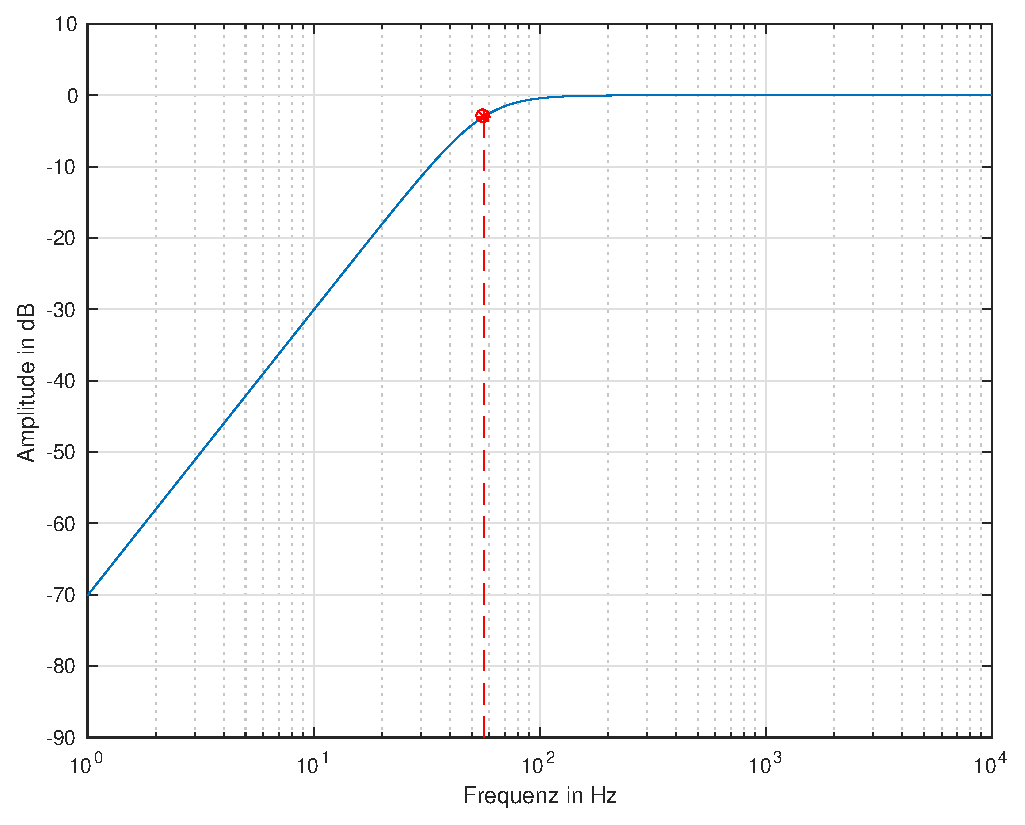
\includegraphics[width=0.7\textwidth]{Figures/Normaler_Frequenzgang.eps}
    \captionsetup{justification=centering}
    \caption{Amplitudenfrequenzgang für V = 68,57 l.\\
    Roter Kreis: Resonanzfrequenz $f_c$. Roter Stern: -3 dB Cutoff-Frequenz.\\
    Resonanz- und Cutofffrequenz fallen zusammen.}
    \label{fig:Normaler_Frequenzgang}
\end{figure}%

Anschließend sollten die Gehäusevolumen $V_{b,3}$ und $V_{b,1}$ ermittelt werden, welche zu einer maximalen Überhöhung des Betragfrequenzgangs von 3 dB bzw. 1 dB respektive führen.
Dies wurde in einem iterativen Prozess umgesetzt.
Die resultierenden Frequenzgänge sind in Abbildung \ref{fig:Ueberhoehung} zu sehen.
Wie in der vorhergehenden Abbildung ist die Resonanzfrequenz $f_c$ mit einem roten Kreis und die -3 dB Cutoff-Frequenz mit einem roten Sternchen markiert.
Der berechnete Wert von $V_{b,3}$ liegt bei 18 Litern mit einer Güte $Q_{ts}$ von 1.32.
Für $V_{b,1}$ wurde ein Wert von 35 Litern und eine Güte von 0.96 errechnet.

\begin{figure}[H]
    \centering
    
    \begin{subfigure}{.49\textwidth}
        \centering
        \caption{1dB Überhöhung für $V_{b,1} = 35$ l}
        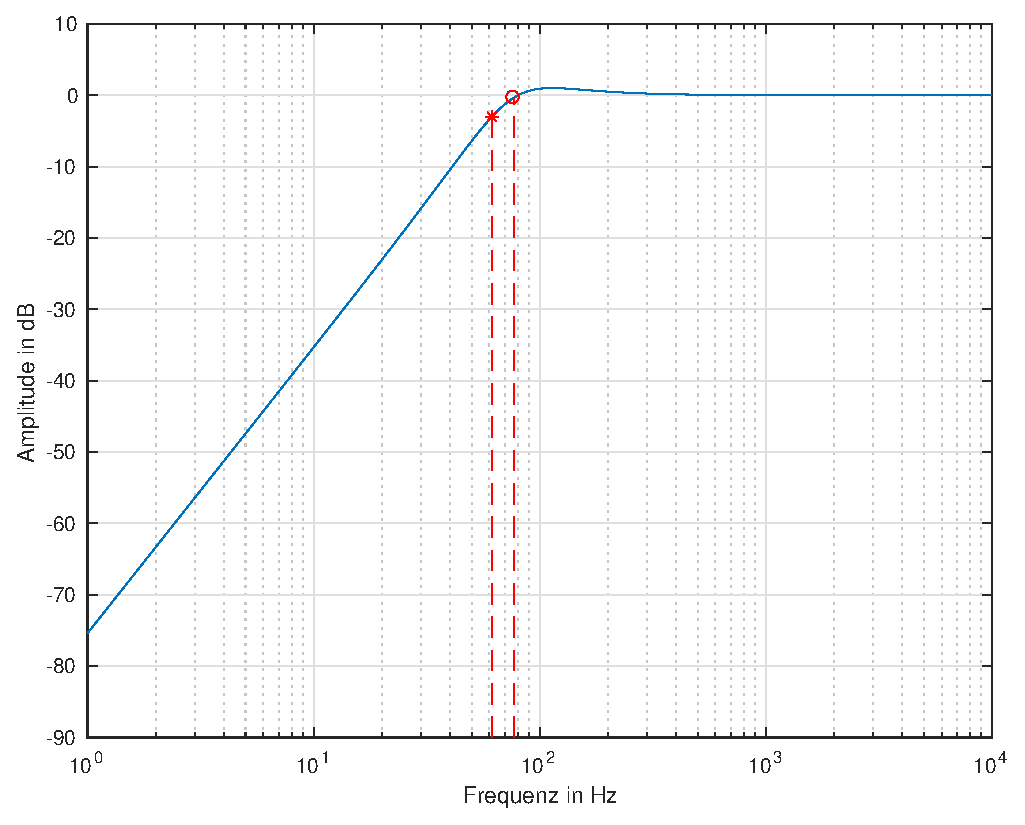
\includegraphics[width=0.85\linewidth]{Figures/Frequenzgang_1dB.eps}
        \label{Frequenzgang_1dB}
    \end{subfigure}
    \begin{subfigure}{.49\textwidth}
        \centering
        \caption{3dB Überhöhung für $V_{b,3} = 18$ l}
        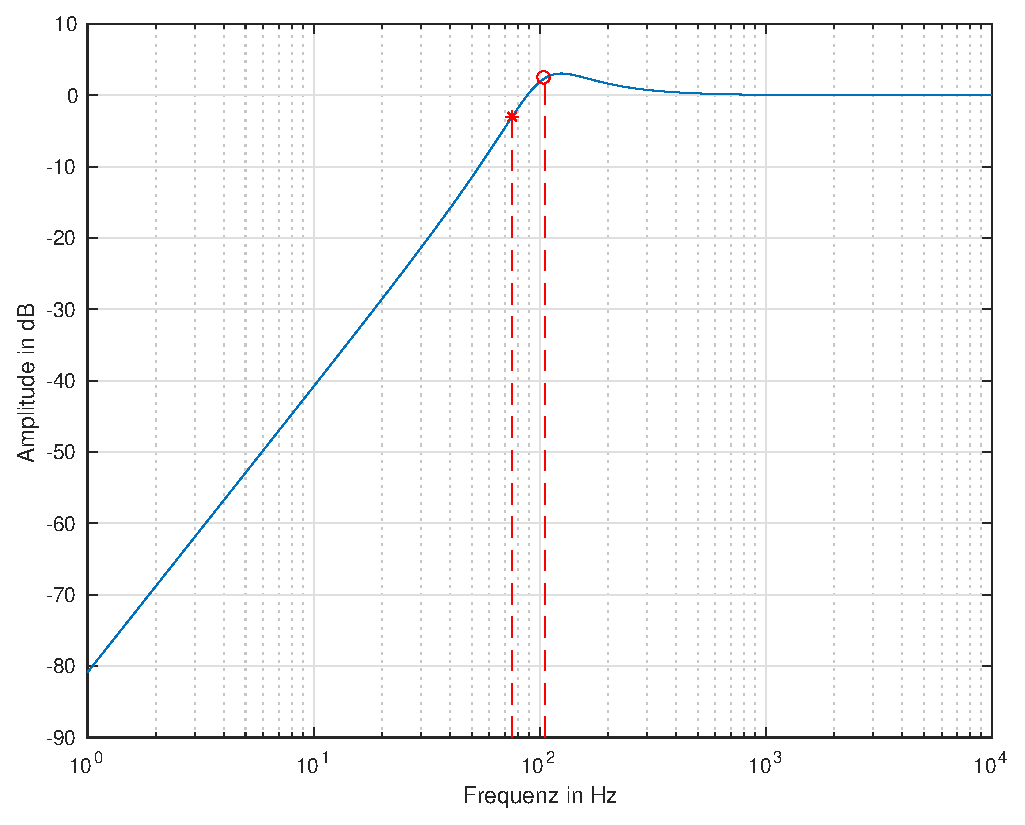
\includegraphics[width=0.85\linewidth]{Figures/Frequenzgang_3dB.eps}
        \label{Frequenzgang_3dB}
    \end{subfigure}
    \captionsetup{justification=centering}
    \caption{Frequenzgänge mit verschiedenen Überhöhungen.\\Rote Kreise: Resonanzfrequenz $f_c$. Rote Sterne: -3 dB Cutoff-Frequenz.}
    \label{fig:Ueberhoehung}
\end{figure}
Aus den verschiedenen Gehäusegrößen ergeben sich verschiedene Vor- und Nachteile aus praktischer, nachrichtentechnischer und verkaufspsychologischer Sicht.
Zunächst sind kleine Gehäuse praktischer, weil sie sich einfacher transportieren lassen und nicht so viel Platz einnehmen, dies kann auch beim Kauf ein ausschlaggebendes Kriterium sein.
Große Gehäuse wiederum können auf Veranstaltungen einen beeindruckenden optischen Effekt hervorrufen. 
Die Größe des Gehäuse hat wie bereits erwähnt und in den Abbildungen \ref{fig:Normaler_Frequenzgang} und \ref{fig:Ueberhoehung} dargestellt zudem einen Effekt auf den Frequenzgang. 
Das große Gehäuse (V = 68,57 l) hat den größten linearen Bereich und keine Überhöhung. 
Es ist damit aus nachrichtentechnischer Sicht optimal, weil alle Frequenzen oberhalb des Abfalls im tiefen Bereich klar wiedergegeben werden. 
Zudem hat dieses Gehäuse den schwächsten Abfall hin zu tiefen Frequenzen, insgesamt werden also tiefe Frequenzen außerhalb des linearen Bereichs lauter wiedergegeben als bei den kleineren Gehäusen.
Dieser Aspekt ist auch verkaufspsychologisch von Vorteil.
Die kleineren Gehäuse hingegen verstärken einen bestimmten Frequenzbereich in der Nähe der Resonanzfrequenz, für viele Zwecke kann dies ausreichend oder sogar erwünscht sein.
Beim Einsatz als Subwoofer will man vor allem den Bassbereich lauter wiedergeben und diesen Bereich vom Bereich höherer Frequenzen trennen.
Der hier analysierte Treiber ist für diesen Effekt allerdings nicht optimal geeignet, weil sein Frequenzgangsmaximum bei zu hohen Frequenzen im Bereich um 100 Hz liegt. 
Treiber mit niedriger Resonanzfrequenz können hingegen Resonanzüberhöhungen bis in den Subbassbereich liefern.
\files{main.m, G.m}